\chapter{Validation, convergence and conservation experiments}
\label{cha:numer-experiments}

In this section we apply the various numerical methods constructed throughout this thesis to some more realistic micromagnetics problems.

The first case examined is a 2D problem without magnetostatics where there is a known wave-like analytical solution for certain initial conditions.
This allows us to test the convergence of the various methods when applied to the full PDE form of the LLG, as well as the geometric integration properties of the IMR.

The second problem is another simple case, but without an analytical solution: a non-uniform applied field is used to induce non-uniform dynamics in a 2D problem without magnetostatics.
This allows us to test geometric integration properties of the IMR in the absence of an analytical solution.

We then show results from the \mumag standard problem \#4 \cite{mumag-website}, which is widely used to test dynamic micromagnetic codes.
This allows us to verify the complete model and to examine the geometric integration properties when the FEM/BEM magnetostatics calculations are included.


\section{Wave-like solution}
\label{sec:numer-exper}

\subsection{Problem definition}
\label{sec:wave-problem-definition}

In this experiment model the wave-like exact solution in 2D, details of this solution are given in \cref{sec:wave-like-solution}.
We solve the LLG without magnetostatics on a two dimensional square domain $\magd = [0,1] \times [0,1]$ with periodic boundary conditions.
In time we simulate the solution in $T = [0, 5]$.
This solution is obtained by setting the initial condition according to \cref{eq:97}:
\begin{equation}
  \begin{aligned}
    m_x(0) &= \sin(c) \cos\bigb{\kvec \cdot \xv}, \\
    m_y(t) &= \sin(c) \sin\bigb{\kvec \cdot \xv}, \\
    m_z(t) &= \cos(c),
  \end{aligned}
\end{equation}
and using $\happ = \zerov$.
The solution parameters used are $\kvec = 2\pi$ (so that the solution is periodic on domains of unit size), $c = 0.1\pi$ and $\dampc = 0.01$.
For the energy conservation experiments $\dampc = 0$ is used instead.

This problem allows us to examine the convergence and geometric integration properties of IMR with the FEM and nodal quadrature.
In particular the existence of an exact solution allows us to easily measure rate of convergence for the various methods.
This allows us to explore the effects of the geometric integration properties of IMR on the accuracy of the solution.


\subsection{Implementation details}
\label{sec:impl-deta}

We use the finite element method as discussed in \cref{sec:galerk-meth-llg} to spatially discretise the LLG equation.
Unless otherwise specified we use a mesh of square elements with $5 \times 2^4$ elements along each edge.
For the evaluation of the resulting integrals both the nodal quadrature discussed in \cref{sec:local-nodal-integr} and standard Gaussian quadrature methods are used.

For time integration the adaptive IMR, TR and BDF2 methods are used with a tolerance of $\toltt = 10^{-5}$ and an initial time step of $\dtn{0} = 10^{-5}$ (significantly smaller than the time step selected by an initial experimental run).
The methods which do not naturally conserve $\abs{\mv}$ (TR and BDF2 methods, and IMR when Gaussian quadrature is used) are run both with and without re-normalisation of the magnetisation.
The re-normalisation process is implemented by setting each nodal value of the magnetisation to $\mv_i = \mv_i/\abs{\mv_i}$ after each time step (after the selection of the next step size to avoid complicating the adaptivity process).

Linearisation is handled using the Newton-Raphson method with newton tolerance set to $\ntol = 10^{-12}$ (unless otherwise specified).
The resulting linear systems are solved using GMRES with an ILU(1) preconditioner as described in \cref{sec:llg-only-system}.

The adaptive IMR integrator, as described in \cref{sec:adaptive-imr}, requires the computation of an explicit time step.
For this step we use the Landau-Lifshitz form of the LLG discretised in exactly the same way as described in \cref{sec:galerk-meth-llg}.
The resulting linear system (involving only a mass matrix) is solved using the method of conjugate gradients preconditioned by the lumped mass matrix (\ie the diagonal matrix of the row sums).
Note that when nodal quadrature is used the mass matrix is a diagonal matrix and so no linear solve is needed (see \cref{sec:nodal-integration}).


\subsection{General results}

An example snapshot of the solution at time $t=??ds$ is shown in \cref{fig:2d-wave-snapshot}.
As time proceeds the wave moves in the $[1,1]$ direction and is simultaneous damped out towards the $\mv = [0,0,1]$ state.

\begin{figure}
  \centering
  
\includegraphics[width=0.8\textwidth]{images/placeholder}
  \caption{Snapshot of the solution at $t=??ds$ (solved using adaptive IMR with nodal integration).}
  \label{fig:2d-wave-snapshot}
\end{figure}

The behaviour of the approximate solutions over time at $\xv = \zerov$ is shown in \cref{fig:2d-wave-time-trace}.
Only results from the methods without re-normalisation are shown because there are no differences distinguishable at the scale of the plot.

The time steps selected by the various algorithms for this problem are also shown in \cref{fig:2d-wave-time-trace}.
The appearance of a jump in the time step size at $t=0$ is due to the algorithms rapidly increasing the time step size from the small initial value to a step size appropriate for the given tolerance.
After an appropriate step size is reached there is a smooth, gradual increase as the solution is damped out.
This is as expected, in particular note that there is no oscillation of the step size with the precessional motion as was observed in \cref{sec:aimr-llgode-numerical-results}.

\begin{figure}
  \centering
  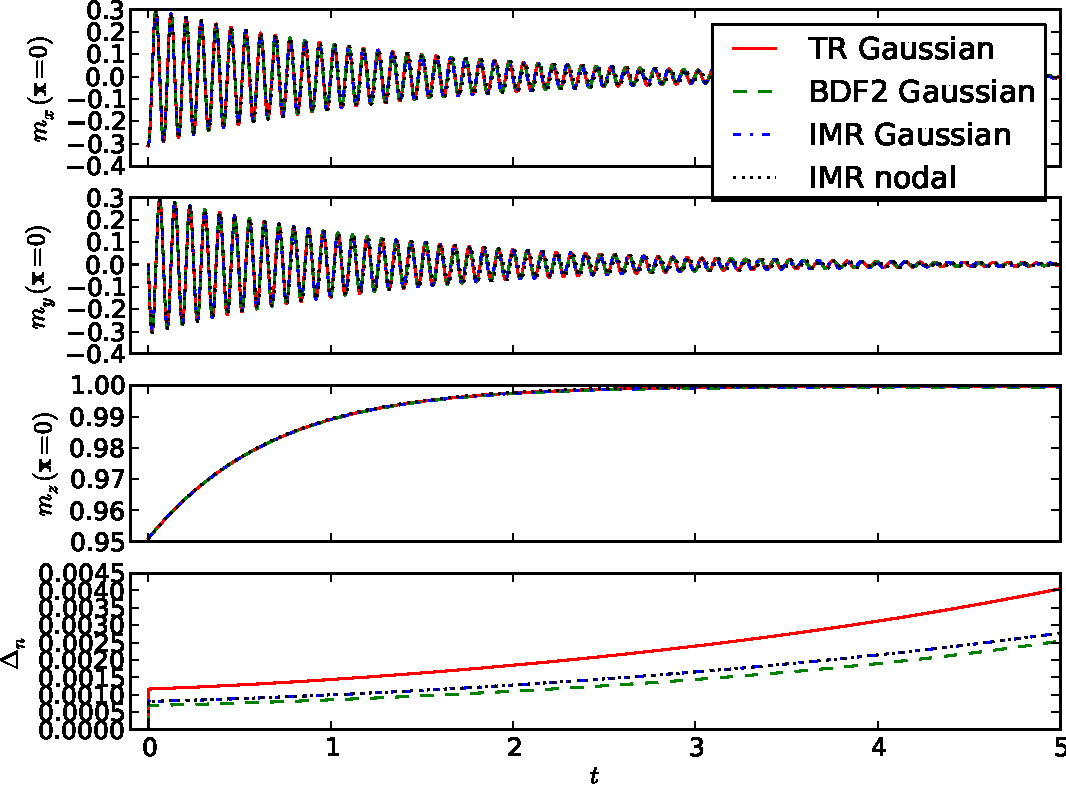
\includegraphics[width=0.9\textwidth]{plots/2d_wave_solution_time_trace/get2oftracevaluesvs-get3oftracevaluesvs-get4oftracevaluesvs-dtsvstimes.pdf}
  \caption{The behaviour of the wave solution at $\xv = \zerov$ over time and the time steps selected by the various adaptive integration schemes without re-normalisation.
The behaviour with re-normalisation is indistinguishable at this scale.}
  \label{fig:2d-wave-time-trace}
\end{figure}


\subsection{Convergence}

Since we have an exact solution for this example we can easily calculate an error norm and plot the convergence as both the time step $\dtn$ and the element edge length $h$ go to zero.
Following the example of Jeong \etal \cite{Jeong2014} we link the time step size to the spatial discretisation size by $\dtn = 0.32h$.
It is important to note that, in contrast to explicit time integration schemes, this coupling of the time and space discretisation parameters is \emph{not} required for stability, it is merely more convenient to experiment with a single parameter than with two independent parameters.
We choose element edge lengths of $h = 1/(5 \cdot 2^n)$ with $n=1,2,3,4,5,6$.
% Larger values of $n$ grow extremely computationally expensive for two reasons: firstly because we choose to reduce the time step and $h$ simultaneously, and so require more solves of larger systems.
% Secondly our iterative linear solver becomes less effective due to the extremely large systems involved ($\sim 10^6$ rows with $n=8$).

In these experiments we always use re-normalisation for schemes which are not expected to naturally conserve $\abs{\mv}$ because in practical applications such schemes would not be used without re-normalisation.

As a first convergence experiment we examine the norm of the error after a single time step
\begin{equation}
  \merr_{,1} = \norm{\mv(\xv_j, t_1) - \mv_{j,1}}_2.
\end{equation}
In this case we expect the convergence (in both space and time) to be second order for all methods.
The results of this experiment are shown in \cref{fig:convergence-one-step},
We see that convergence is indeed second order for all methods and that the accuracy for the BDF2 scheme is a roughly constant factor worse than with other schemes.
We also see that the use of nodal quadrature results in an error increase by a small constant factor.
This indicates that the geometric integration properties of IMR with nodal quadrature give no benefit for a single time step, as would be expected.
\begin{figure}
  \centering
  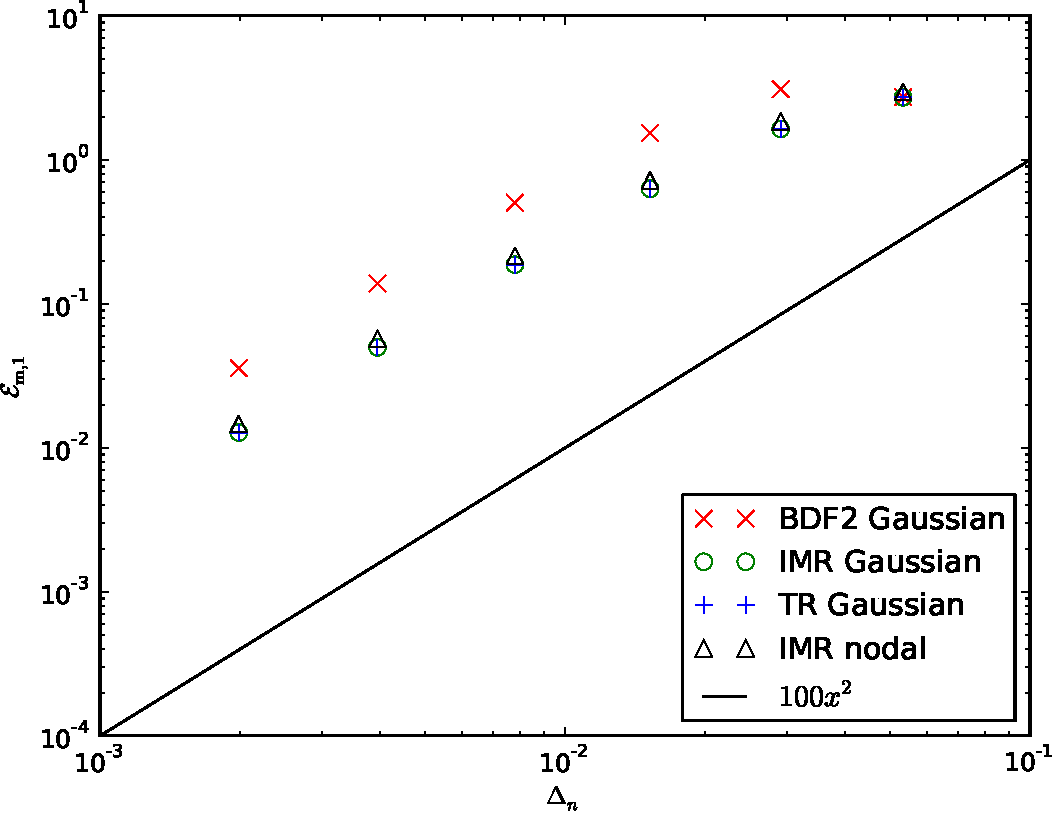
\includegraphics[width=0.9\textwidth]{plots/2d_wave_solution_convergence_long_time/firstoferrornormsvsfakemeanofdts.pdf}
  \caption{Convergence in the error norm $\errmpde{}$ after a single step of time integration.}
  \label{fig:convergence-one-step}
\end{figure}



We also wish to examine a norm of the error after a large number of time steps, so for the rest of the experiments in this section we examine the integral over $T = [0, 5]$ of the error norm.
However, reaching the levels of convergence required for $\errmpde$ to be meaningful is difficult because the ``worst case'' for the norm is that the approximated magnetisation is out of phase with the exact solution (\ie the error norm is bounded).
A plot of the time integral of $\errmpde$ is shown in \cref{fig:convergence-one-step}, as expected no convergence is seen until $n=5$ for IMR and TR, no convergence at all is seen for BDF2.
\begin{figure}
  \centering
  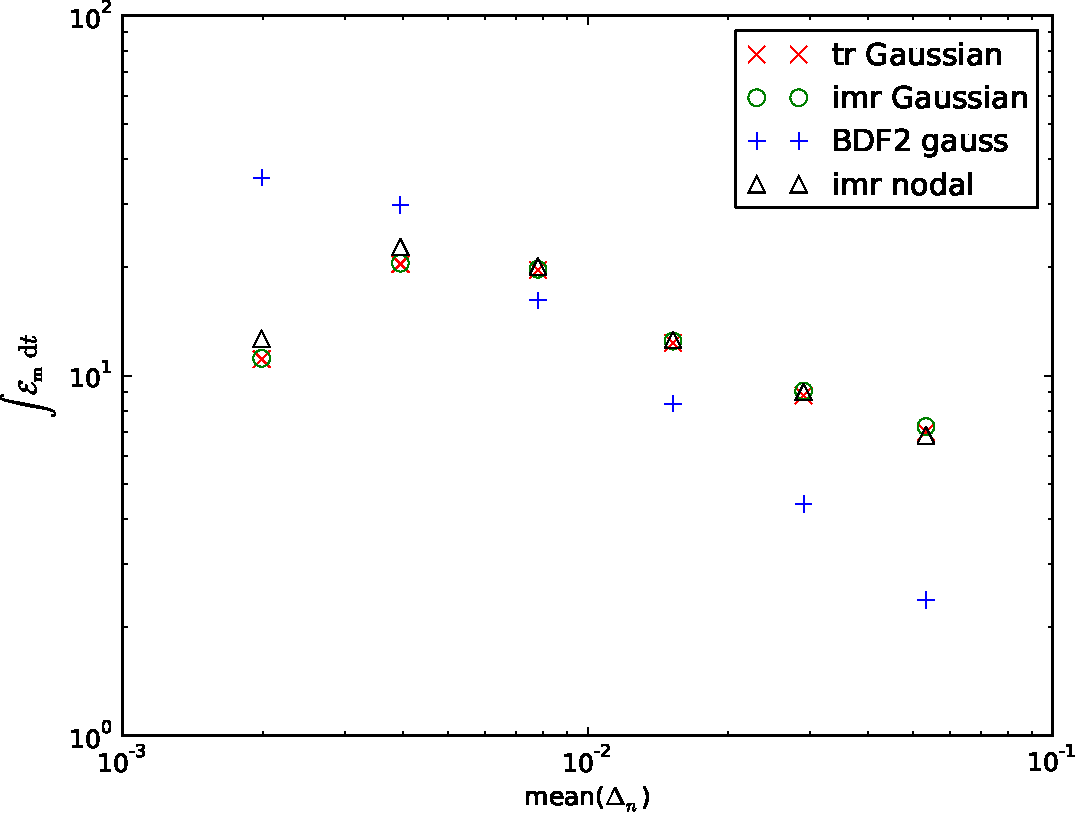
\includegraphics[width=0.9\textwidth]{plots/2d_wave_solution_convergence_long_time/errornormintegralvsmeanofdts.pdf}
  \caption{Convergence of $\intt{\errmpde}$, where $T=[0,5]$, as $h$ and $\dtn$ are simultaneously decreased.}
  \label{fig:convergence-long-time-full-norm}
\end{figure}

To obtain more meaningful results we introduce alternative error norms which allow better measures of the error even for approximate solutions which are out of phase with the exact solution.
Our first such error norm measures the deviation of $m_z$ from the exact value
\begin{equation}
  \errmz = \max_j \abs{m_{z,j,k} - m_z(t_n)},
\end{equation}
note that the exact value of $m_z$ is not a function of $\xv$ and so it is sufficient to take the maximum value.
This error norm measures the level of over/under damping caused by the approximation.

The convergence results for the time integral of the error norm $\errmz$ are shown in \cref{fig:convergence-long-time-full-norm}.
We again see second order convergence behaviour for all methods.
The BDF2 method takes additional time to reach the asymptotic convergence behaviour, and has around an order of magnitude more error than the other methods.
Also note that there is no significant difference between IMR with nodal quadrature (which conserves $\abs{\mv}$) and IMR with Gaussian quadrature (in which $\mv$ is re-normalised), indicating that geometric integration offers no significant benefits in this case.
\begin{figure}
  \centering
  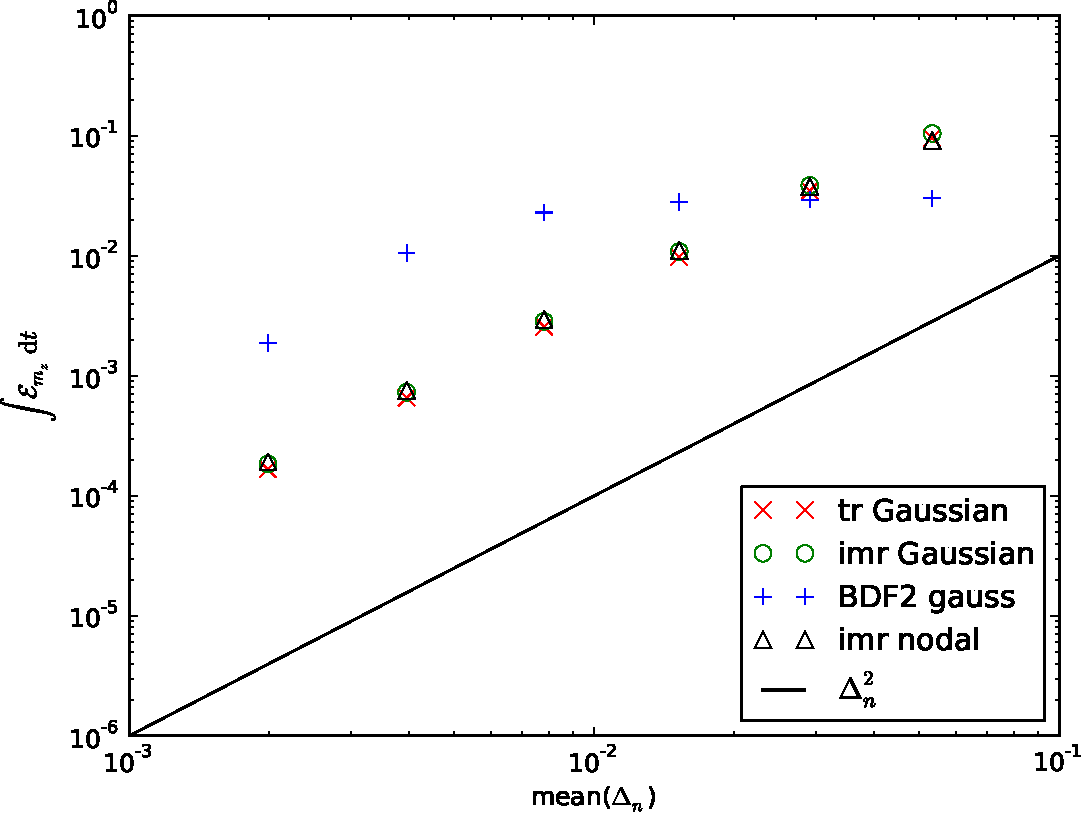
\includegraphics[width=0.9\textwidth]{plots/2d_wave_solution_convergence_long_time/auxerr1integralvsmeanofdts.pdf}
  \caption{Convergence of $\intt{\errmz}$, where $T=[0,5]$, as $h$ and $\dtn$ are simultaneously decreased.}
  \label{fig:convergence-long-time-mz-norm}
\end{figure}


Our next error norm aims to measure the error in the frequency of the wave.
It is
\begin{equation}
  \begin{aligned}
    \errphase &= \abs{\psi_{n,0} - \psi(t_n, 0)}, \\
    &= ??ds,
  \end{aligned}
\end{equation}
where $\psi(t_n, 0) = ...$ is the analytical phase of the wave at $\xv = \zerov$, and $\psi_{n,0}$ is the corresponding phase in approximate solution.
The convergence results with this error norm are shown in \cref{fig:convergence-long-time-phase-norm}.
Unfortunately it appears that this error norm is not much better than $\errmpde$ in terms of measuring the error outside of the asymptotic regime, and we can only draw the same conclusions as for that example.
\begin{figure}
  \centering
  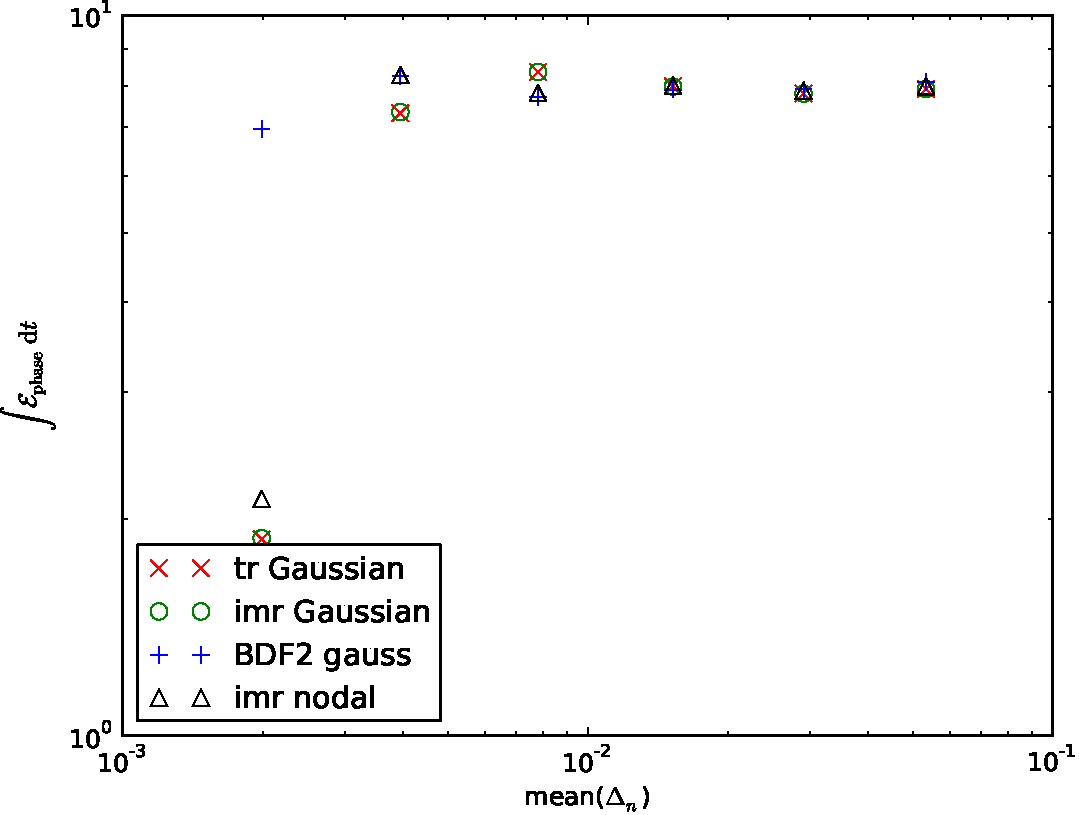
\includegraphics[width=0.9\textwidth]{plots/2d_wave_solution_convergence_long_time/auxerr0integralvsmeanofdts.pdf}
  \caption{Convergence of $\intt{\errphase}$, where $T=[0,5]$, as $h$ and $\dtn$ are simultaneously decreased.}
  \label{fig:convergence-long-time-phase-norm}
\end{figure}



\subsection{Geometric integration properties}
\label{sec:2d-wave-results-cons-prop}

We now examine the error in magnetisation length in the approximations generated by each of the time integration schemes (without re-normalisation).
\Cref{fig:mean-ml-error-2d} shows the evolution of the maximum (over all nodes) of the error in magnetisation length.
When using IMR with nodal quadrature the magnetisation length error remains extremely small but for other methods the error rapidly grows to around $\order{10^{-4}}$ and remains there.
\begin{figure}
  \centering
  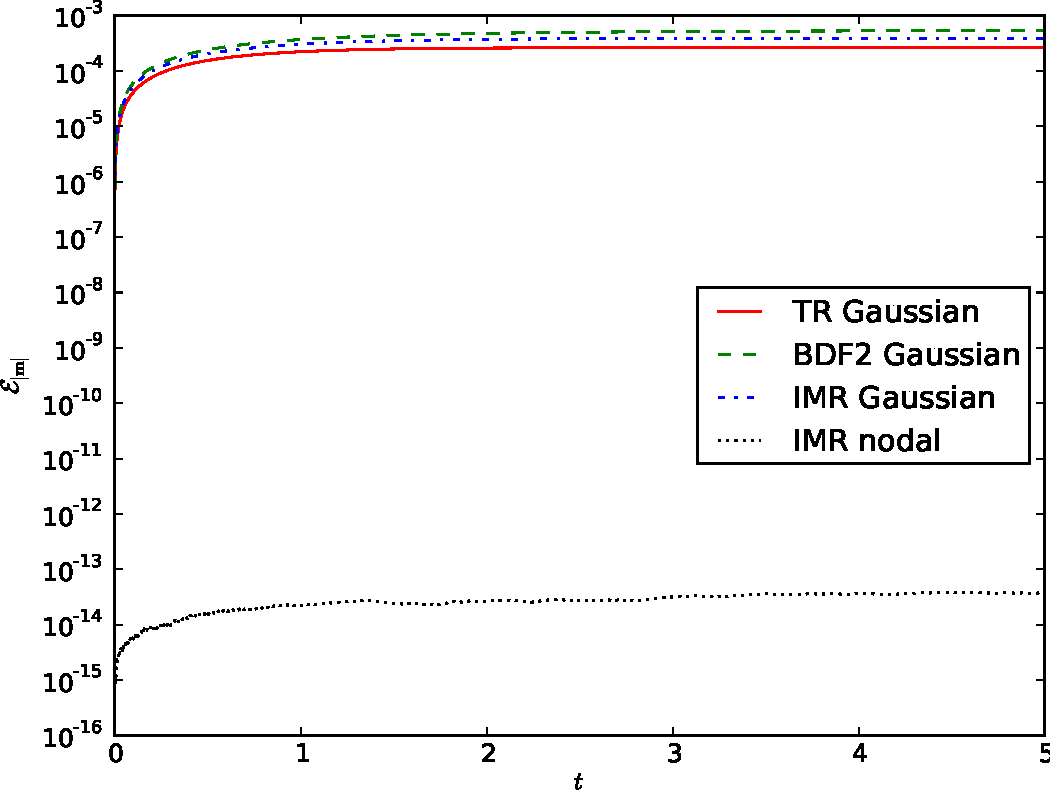
\includegraphics[width=0.8\textwidth]{plots/2d_wave_solution_m_length/mlengtherrormaxesvstimes.pdf}
  \caption{Evolution of the maximum error of nodal magnetisation lengths with various time integrators and quadratures.}
  \label{fig:mean-ml-error-2d}
\end{figure}

We next examine the energy conservation properties of the various schemes for the wave solution with $\dampc = 0$.
The only energy involved is the exchange energy, which can be calculated using \cref{eq:nd-e-ex}.
Note that these integrals can be evaluated exactly by any quadrature because $\grad \mv$ is a constant inside each element.
The results are shown in \cref{fig:energy-error-2d}, interestingly we see that IMR with Gaussian quadrature and TR both conserve energy in a similar manner to IMR with nodal quadrature.
This is likely due to some property of the exact solution, and does not appear to be the case in general (see \cref{sec:non-uniform-applied}).
\begin{figure}
  \centering
  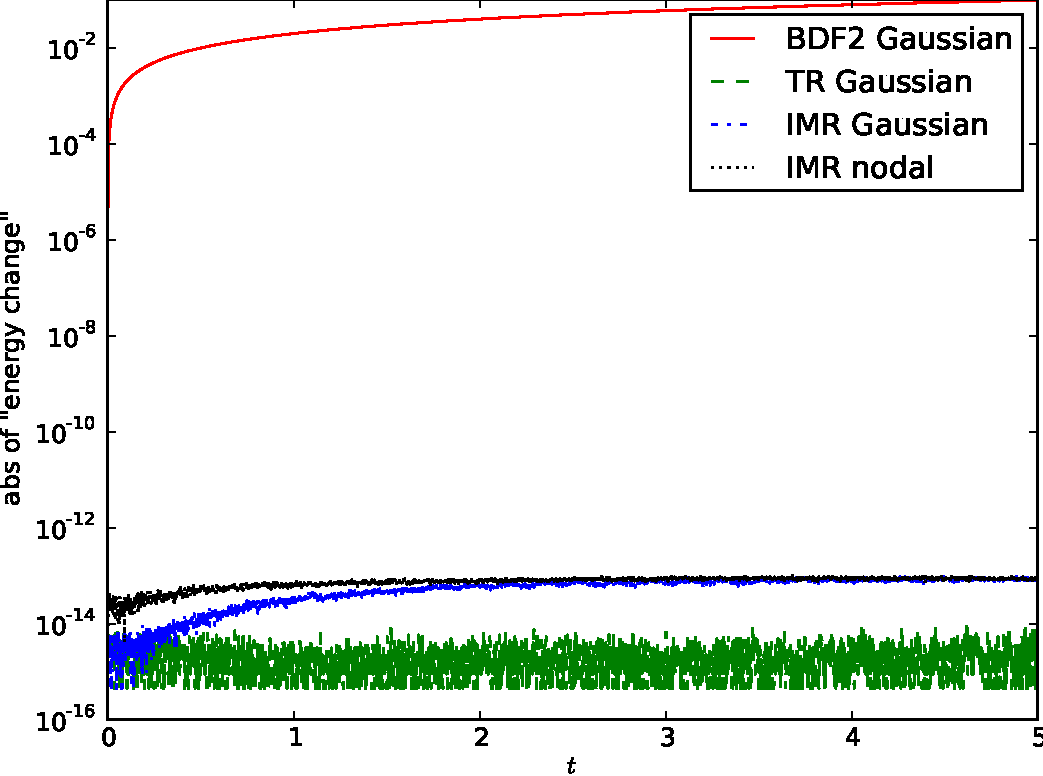
\includegraphics[width=0.8\textwidth]{plots/2d_wave_solution_energy/absofenergychangevstimes}
  \caption{Evolution of the error in energy in the undamped case with various time integration methods and quadrature schemes.}
  \label{fig:energy-error-2d}
\end{figure}


\subsection{Effect of Newton tolerance}
\label{sec:effect-newt-toler-m-conservation}

Since the non-linear residual \cref{eq:weak-llg} used in the derivation of the conservation properties for energy and $\abs{\mv}$ is only true up to the accuracy of the linearisation method we would expect to see some effect on the conservation properties when modifying this accuracy.
In our implementation the Newton-Raphson method is used for linearisation, so the relevant measure of accuracy is the Newton tolerance, $\ntol$.

The obvious experiment to carry out would be to vary the Newton tolerance and examine how the error in $\abs{\mv}$ is affected.
However the Newton-Raphson method converges extremely quickly meaning that the final residual is often many orders of magnitude smaller than the tolerance, this would hide any corrolation between the tolerance and the error.
Instead we plot the error against the \emph{actual} converged residual norm (specifically: the mean over all time steps of $\norm{\rv}_\infty$ after the Newton method has converged for that time step).
In order to generate a variety of converged residual norms we run the experiment with a range of parameters: $\ntol = 10^{8}, 10^{9}, 10^{10}, 10^{11}, 10^{12}$; $\toltt = 10^{3}, 10^{4}, 10^{5}$; $\dampc = 1, 0.001, 0$; and $h = 0.05, 0.025, 0.0125$.
We only calculate in time in $T = [0, 1]$ due to the volume of computations required.
The results are shown in \cref{fig:ml-error-2d-nodal-newton-tests}, there is a clear correlation between small residuals and small $\abs{\mv}$ error.
A similar result is seen in \cref{fig:energy-error-2d-nodal-newton-tests} for the energy conservation property when $\dampc = 0$.

\begin{figure}
  \centering
  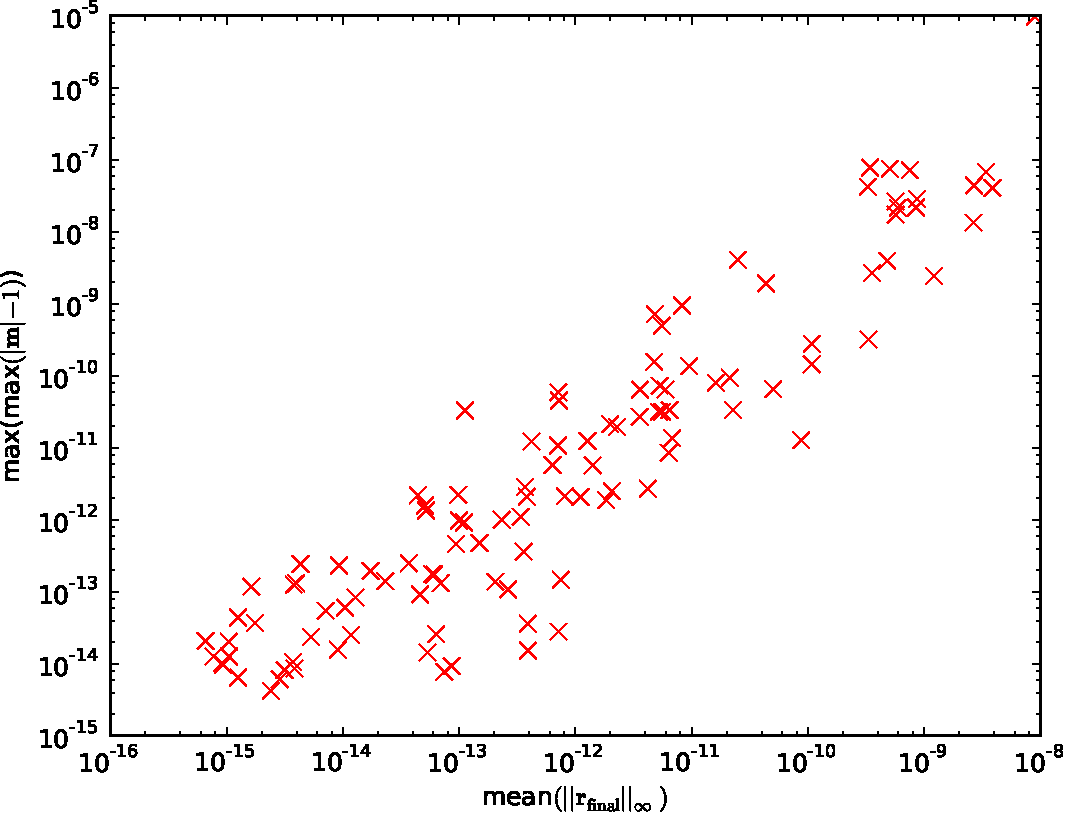
\includegraphics[width=0.8\textwidth]
  {plots/2d_wave_solution_m_length_newton_res/maxofmlengtherrormaxesvsmeanminofnewtonresiduals.pdf}
  \caption{Corrolation between maximum (over all nodes and all time steps) error of nodal magnetisation lengths and the mean (over time) of the converged Newton residual norm in the 2D wave example solved using adaptive IMR and nodal quadrature.}
  \label{fig:ml-error-2d-nodal-newton-tests}
\end{figure}


\begin{figure}
  \centering
  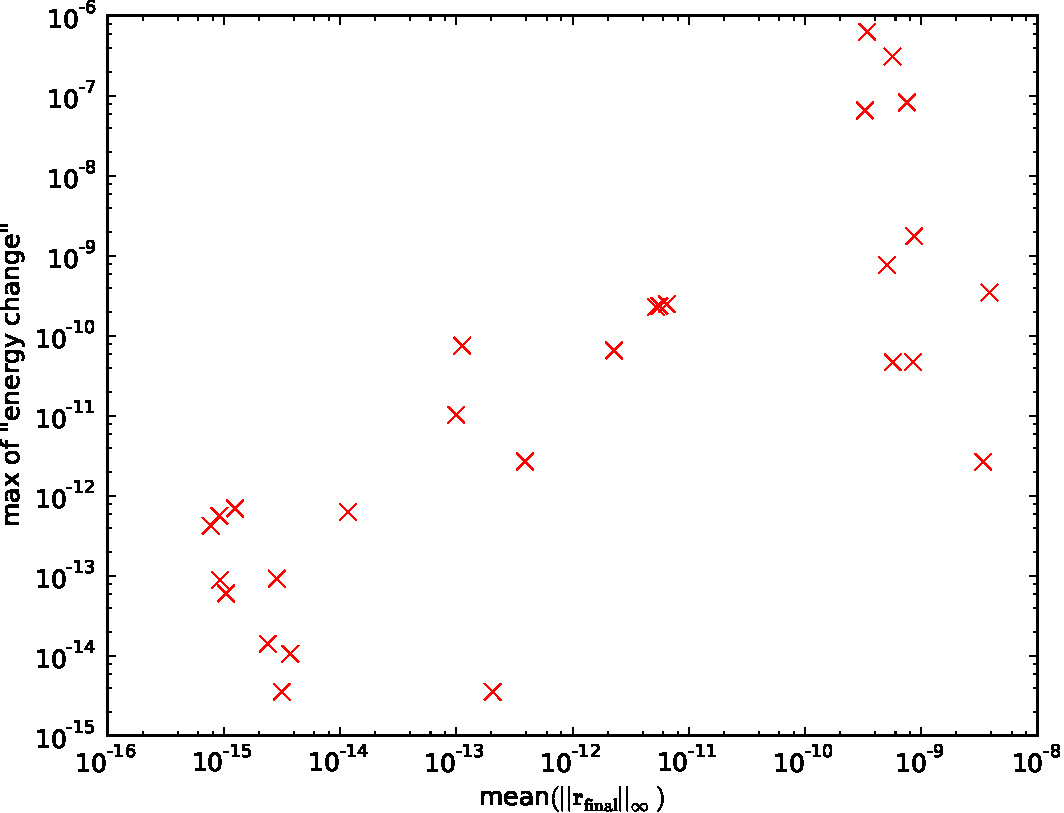
\includegraphics[width=0.8\textwidth]
  {plots/2d_wave_solution_energy_newton_res/maxofenergychangevsmeanminofnewtonresiduals.pdf}
  \caption{Corrolation between the maximum (over time) of the error in energy and the mean (over time) of the converged Newton residual norm in the undamped 2D wave example solved using adaptive IMR and nodal quadrature.}
  \label{fig:energy-error-2d-nodal-newton-tests}
\end{figure}



\subsection{Conclusions}

We have shown that the methods used have the expected convergence and time step selection properties.
We also observed that the asymptotic accuracy of the BDF2 method is lower than the TR or IMR methods by a moderately sized constant factor.

We have also shown that the geometric integration properties of IMR persist in a weak form FEM model when used with a nodal quadrature scheme.
Finally we have shown that these properties are linked to the accuracy of the non-linear solver, as predicted in \cref{sec:nodal-integration}.

We have also observed unexpected geometric integration properties when IMR with Gaussian quadrature or TR are used.
It is expected that this is a property of the analytical solution rather than the methods themselves, this will be tested in the next section.

Since all time integration schemes except for BDF2 showed some geometric integration properties the effect of such properties on the overall error cannot be analysed using this example.


\FloatBarrier
\section{Non-uniform applied field example}
\label{sec:non-uniform-applied}

In \thisref{sec:non-uniform-applied} we construct a problem which is non-uniform in space without the involvement of the magnetostatic field by applying a non-uniform applied field.
This will allow us to examine whether the anomalous geometric integration properties observed in the previous section are related to the analytical solution.

This experiment also reveals some odd behaviour on meshes of triangular elements.

\subsection{Problem definition}

We solve the LLG without magnetostatics on a two dimensional square domain $\magd = [0,5] \times [0,5]$ with Neumann boundary conditions.
In time we simulate the solution in $T = [0, 5]$.

We use a uniform initial condition $\mv = [1, 1, 0]/\sqrt{2}$ with a non-uniform applied field
\begin{equation}
  \happ =
  \begin{cases}
    1.1 (1 -  x) & x  < 1, \\
    0 & \mathrm{otherwise}.
  \end{cases}
\end{equation}
As before we use $\dampc = 0.01$ except for energy conservation experiments which use $\dampc = 0$.
The implementation details of this example are exactly as described in \cref{sec:impl-deta} except that we also use meshes of triangular elements.
The structure of the triangular element mesh is equivalent to the square element case except that each element is divided in two diagonally.

??ds describe physics?

% \subsection{General results}

% time trace

% \begin{figure}
%   \centering
%   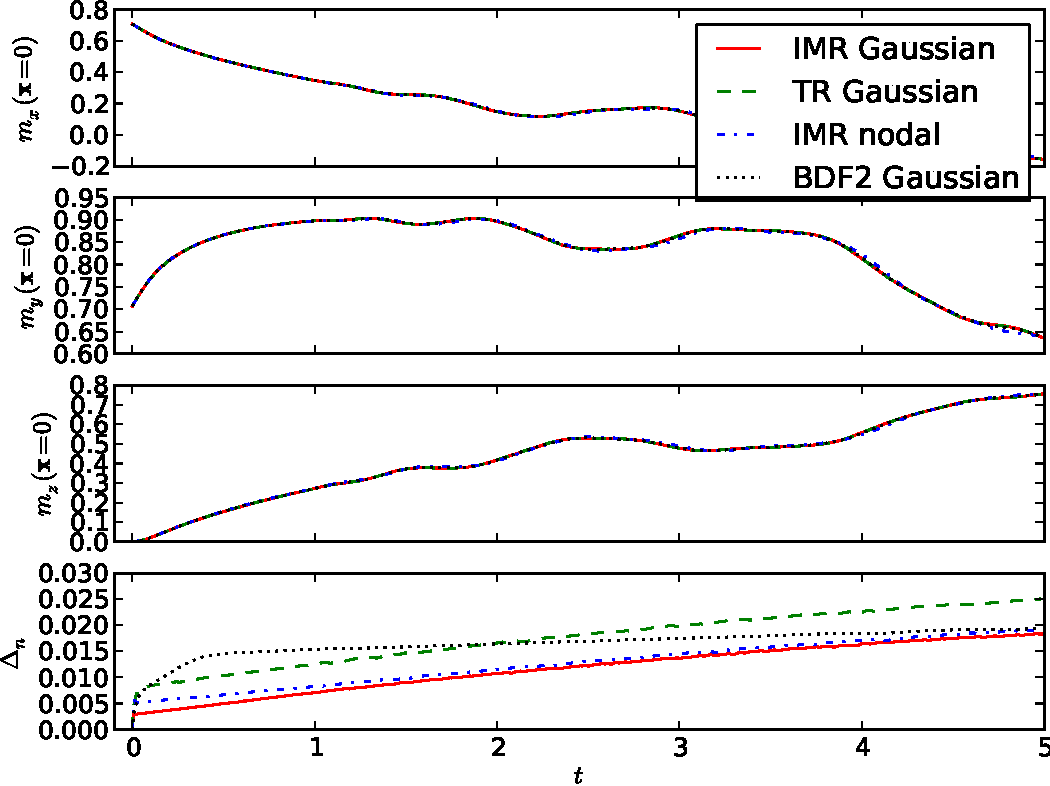
\includegraphics[width=0.8\textwidth]{plots/nonuniform-h-trace/get2oftracevaluesvs-get3oftracevaluesvs-get4oftracevaluesvs-dtsvstimes.pdf}
%   \caption{Behaviour of the mean magnetisation over time for the non-uniform applied field example.}
%   \label{fig:nonuniform-h-time-trace}
% \end{figure}


% snapshot?


\subsection{Geometric Integration properties}


The evolution of the magnetisation length for this experiment is shown in \cref{fig:nonuniform-h-ml-error}, we see that in this case only IMR with nodal quadrature conserves $\abs{\mv}$ as expected.
The same is true for the energy conservation with zero damping, as shown in \cref{fig:nonuniform-h-energy-error}.

\begin{figure}
  \centering
  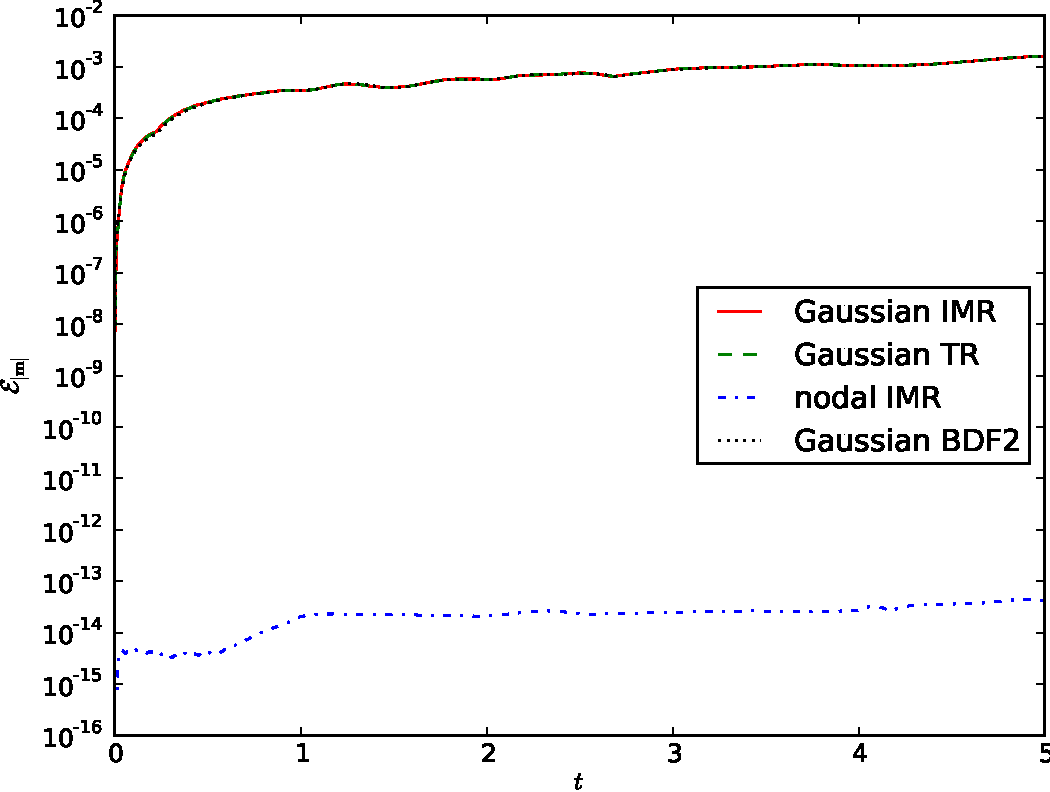
\includegraphics[width=0.8\textwidth]
  {plots/nonuniform-h-ml/mlengtherrormaxesvstimes.pdf}
  \caption{Evolution of the maximum error of nodal magnetisation lengths with various time integrators and quadratures for the non-uniform applied field example.}
  \label{fig:nonuniform-h-ml-error}
\end{figure}


\begin{figure}
  \centering
  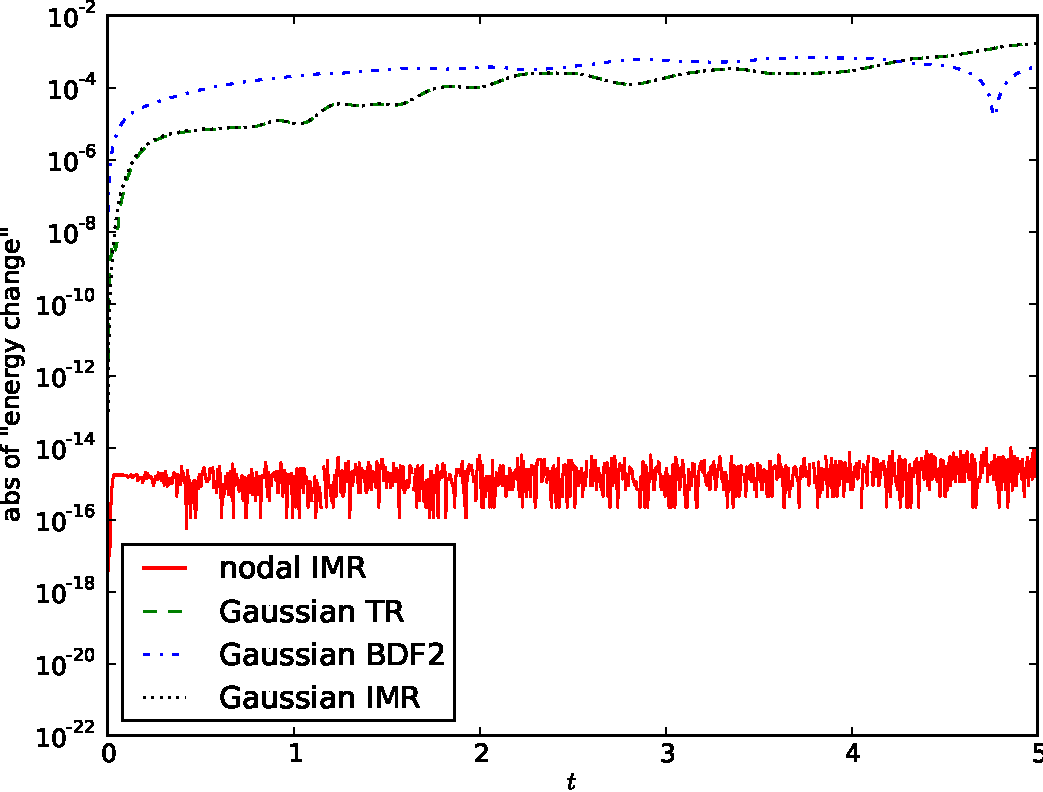
\includegraphics[width=0.8\textwidth]
  {plots/nonuniform-h-energy-change/absofenergychangevstimes.pdf}
  \caption{Evolution of the error in energy in the undamped case with various time integration methods and quadrature schemes for the undamped non-uniform applied field example.}
  \label{fig:nonuniform-h-energy-error}
\end{figure}




\subsection{Triangular meshes}

Finally we show some anomalous results when a mesh of triangular elements is used.
The evolution of $\abs{\mv}$ is shown in \cref{fig:ml-error-triangle-mesh}.
We see that the $\abs{\mv}$ conservation property of IMR with nodal quadrature fails on triangular elements.
Similarly the conservation of energy (with $\dampc = 0$) fails, as shown in \cref{fig:energy-error-triangle-mesh}.
Our other experiments show this issue for a variety of other cases including 3D problems with tetrahedral elements, but not including the wave solution example.

We do not have an explanation for this effect.
However it should be noted that the non-conservation effects are small enough that they would not be noticed if the numerical experiments were run with a loose non-linear solver tolerance, such as used in \eg \cite{Bartels2006}.

\begin{figure}
  \centering
  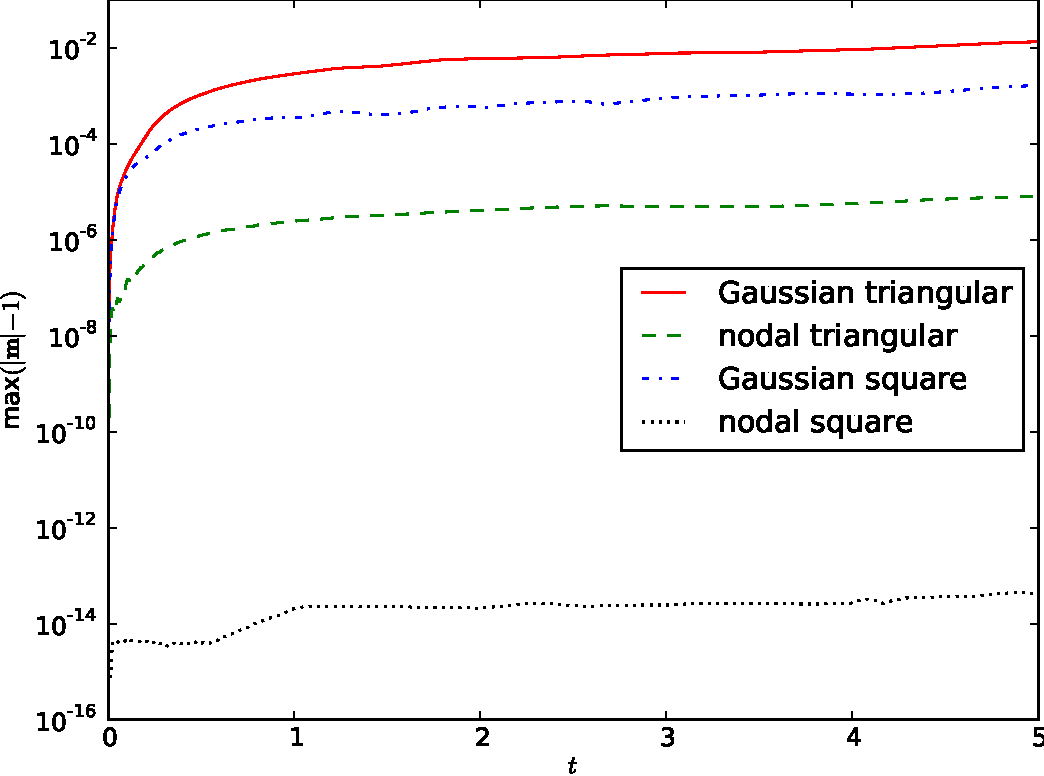
\includegraphics[width=0.8\textwidth]
  {plots/nonuniform-h-triangles-ml/mlengtherrormaxesvstimes.pdf}
  \caption{Maximum error of nodal magnetisation lengths with IMR for the non-uniform applied field example.
Results with other time integration schemes are similar to those for IMR with Gaussian quadrature for both element types.}
  \label{fig:ml-error-triangle-mesh}
\end{figure}

\begin{figure}
  \centering
  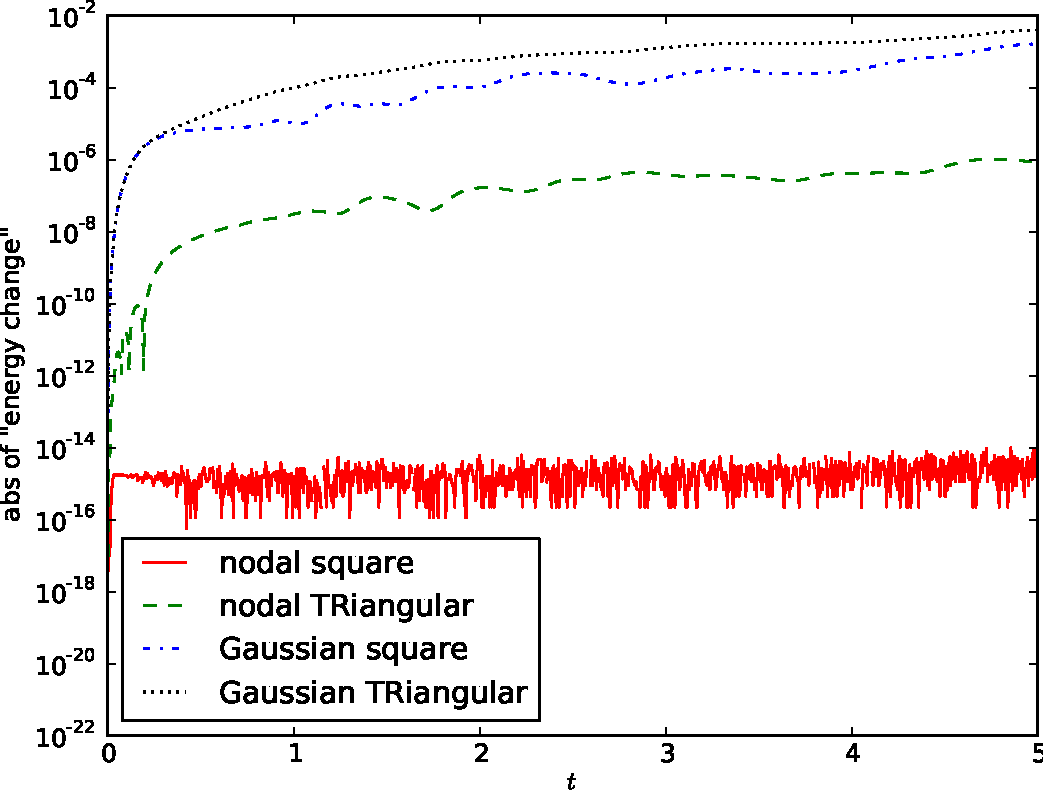
\includegraphics[width=0.8\textwidth]
  {plots/nonuniform-h-triangles-energy-error/absofenergychangevstimes.pdf}
  \caption{Error in energy with IMR for the non-uniform applied field example without damping.
 Results with other time integration schemes are similar to those for IMR with Gaussian quadrature for both element types.}
  \label{fig:energy-error-triangle-mesh}
\end{figure}

\subsection{Conclusions}

We have found that the wave exact solution example is in some sense ``too easy'' and does not provide a rigorous test of geometric integration properties: IMR with Gaussian quadrature and TR do not conserve energy or $\abs{\mv}$ in general.

We have also shown an example of a problem where our implementation of IMR with nodal quadrature unexpectedly \emph{does not} conserve energy or $\abs{\mv}$ when used with a mesh of triangular elements.


% Don't allow floats from last section into this one
\FloatBarrier
\section{The \mumag standard problem \#4}

The \mumag standard problem \#4 \cite{mumag-website} is the problem most widely used to test implementations of dynamic micromagnetic models.
It involves modelling the reversal of an extremely thin cuboid film of permalloy-like material under two different applied fields.
Unfortunately FEM/BEM magnetostatic calcultations are extremely unsuited to thin film problems: the dense BEM matrix size is proportional to the number of nodes on the boundary and in a thin film every single node is on the boundary.
Additionally the key benefit of FEM/BEM (accurate resolution of complex geometries) is not required since the film is a simple cuboid.
However, since there are no other widely studied test problems and there are no problems with both magnetostatics and exchange for which an analytical solution is known, we use the standard problem to verify our implementation.


\subsection{Problem specification}

The magnetic domain is a sheet of magnetic material $500 \times 125 \times 3$nm with material parameters
\begin{equation}
  \begin{aligned}
    A &= 1.3\E{-11} \text{J/m}, \\
    M_s &= 8.0\E{5} \text{A/m}, \\
    \Kone &= 0.0, \\
    \gymagc &= 2.211 \E{5} \text{m/As}, \\
    \dampc &= 0.02.
  \end{aligned}
\end{equation}
The simulation is run with two different applied fields:
\begin{equation}
  \begin{aligned}
    \happ_1 = [-24.6, 4.3, 0.0] \E{-3}\text{A/m}, \\
    \happ_1 = [-35.5, -6.3, 0.0] \E{-3}\text{A/m}, \\
  \end{aligned}
  \label{eq:mumag-h-app}
\end{equation}
where we have converted from the magnetic flux intensity specified by the \mumag website to a magnetic field by dropping the factor of $\mu_0$.
The initial condition is the S-state given by slowly relaxing the magnetisation from the state created by a saturating field in the $[1,1,1]$.

The magnetic parameters result in a magnetostatic exchange length (and unit length in our simulations) of
\begin{equation}
  l_{\text{ex}} = \sqrt{\frac{2A}{\mu_0 M_s^2}} = 5.6858\text{nm},
\end{equation}
hence the normalised dimensions are approximately $87.94 \times 21.98 \times 0.53$.
Our unit time is
\begin{equation}
  t_{\text{unit}} = \frac{1}{\gymagc M_s} = 5.653\text{ps}.
\end{equation}
The normalised applied fields are simply the fields given in \cref{eq:mumag-h-app} divided by $M_s = 8.0\E{5}$.


\subsection{Implementation details}

We use the FEM to spatially discretise the LLG equation and the Newton-Raphson method to solve the resulting non-linear systems as described in \cref{cha:numer-experiments}.
The hybrid FEM/BEM method, described in \cref{sec:hybr-finit-elem}, is used for magnetostatic calculations.
For the coupling of LLG equation with the magnetostatic calculations we use both the monolithic and semi-implicit methods discussed in \cref{sec:solution-strategies}.
The solution of the monolithic linear system is done using the fully iterative preconditioner $\inexact{\precc}$, it turns out that for thin film problems the ILU-1 approximation to the LLG block, $\Fm$, is effective.
The decoupled systems resulting from the semi-implicit method are solved using the methods described in \cref{sec:llg-only-system}.

Both Gaussian quadrature and the nodal quadrature are used.
The TR, BDF2 and IMR adaptive time integration schemes (see \cref{sec:adapt-impl-midp,sec:aimr-implementation}) are tested.
Re-normalisation of the magnetisation is also tested for those schemes which do not naturally conserve $\abs{\mv}$.

As previously mentioned the adaptive IMR requires an explicit time step for the estimation of the error.
This is implemented as described in \cref{sec:impl-deta}.
No coupling with the FEM/BEM calculations is required for this explicit step because only the value of the magnetostatic potential at the previous time step is required (and this is already known from the IMR calculations of the previous step).

A structured mesh consisting of cuboid elements is used due to the simple geometry of the problem and the fact that we have observed issues with geometric integration on tetrahedral elements.
In the $z$ direction (out of the thin film plane) a single layer of elements is used at all refinements.
This is a standard approach, and is expected to give acceptable resolution because the exchange length of the material (the length scale over which the magnetisation can vary) is around twice the thickness.
The number of elements along the $x$ and $y$ axes, denoted $n_x$ and $n_y$, is varied but the ratio is fixed as $n_x = (500/125) n_y$ so that the element edge lengths in each direction are identical.
We use $n_x=75,100,125$, which gives edge lengths of 1.17, 0.89 and 0.70 exchange lengths respectively.

The Newton tolerance is fixed at $\ntol = 10^{-11}$, the adaptive integrator tolerance is $\toltt = 10^{-5}$ and the initial time step is $\dtx{0} = 10^{-4}$.
% We cap the time step at $\dtx{\text{max}} = 4.5$ to avoid issues with linear and solver converge at extremely large time steps.


To generate the initial S-state we run the simulation for 300 time units starting from the state $\mv=[1,1,1]$ with $\dampc = 1.0$ and the applied field
\begin{equation}
  \happ(t) =
  \begin{cases}
    10 (1- \frac{t}{100}) & t < 100, \\
    0 & t \geq 100.
  \end{cases}
\end{equation}
The time integrator history data is then set such that it has been in this state forever and the time step sizes are set to the initial value.
The relevant applied field as specified in the problem is then set and the simulation is continued.
The initial condition is always generated using the same numerical methods as are used in the simulation.

Note that with $\dampc = 1$ the time scale for the magnetisation to fully relax is $\sim 1$, \footnote{Relaxation with $\dampc = 1$ takes one precession cycle and our time units are normalised to the time for a precession cycle driven by a field of strength $M_s$.} with $\dampc \sim 0.01$ the time scale is $\sim 1000$ (see \eg \cref{fig:imr-llg-ode}).
So the simulated time allowed for relaxation to the initial condition is sufficiently long to be considered ``slow'' despite the fact that it is much shorter than the simulated time for the dynamics calculations.



\subsection{General results}

??Ds rerun with longer relaxation time...

For this problem we find that without either re-normalisation or geometric integration the time steps selected by the adaptive algorithms become unacceptably small (\ie the error becomes large).
Hence these cases were not run until completion and are not included in the results.

In \cref{fig:intial-mumag4} we show the initial S-state, as generated by IMR with nodal quadrature.
\begin{figure}
  \centering
  
\includegraphics[width=0.8\textwidth]{images/placeholder}
  \caption{Initial S-state as generated by... ??ds}
  \label{fig:intial-mumag4}
\end{figure}

Next we show the results required for the standard problem: the mean magnetisation for the two fields in \cref{fig:nmag-comparison-mumag4-field1,fig:nmag-comparison-mumag4-field2}.
The results agree reasonably well with the results obtained by d'Aquino, except for the height of the second peak when field 2 is used.

The same plots show the time step selection behaviour.
During relaxation: large value initially, decreasing as the field decreases and the relaxation happens, then very large once the field is gone.
During the dynamics: reasonably large value initially, decreasing around the time of the first switch then steadily increasing as the oscillations are damped out.
The behaviour for the second field is essentially the same.

\begin{figure}
  \centering
  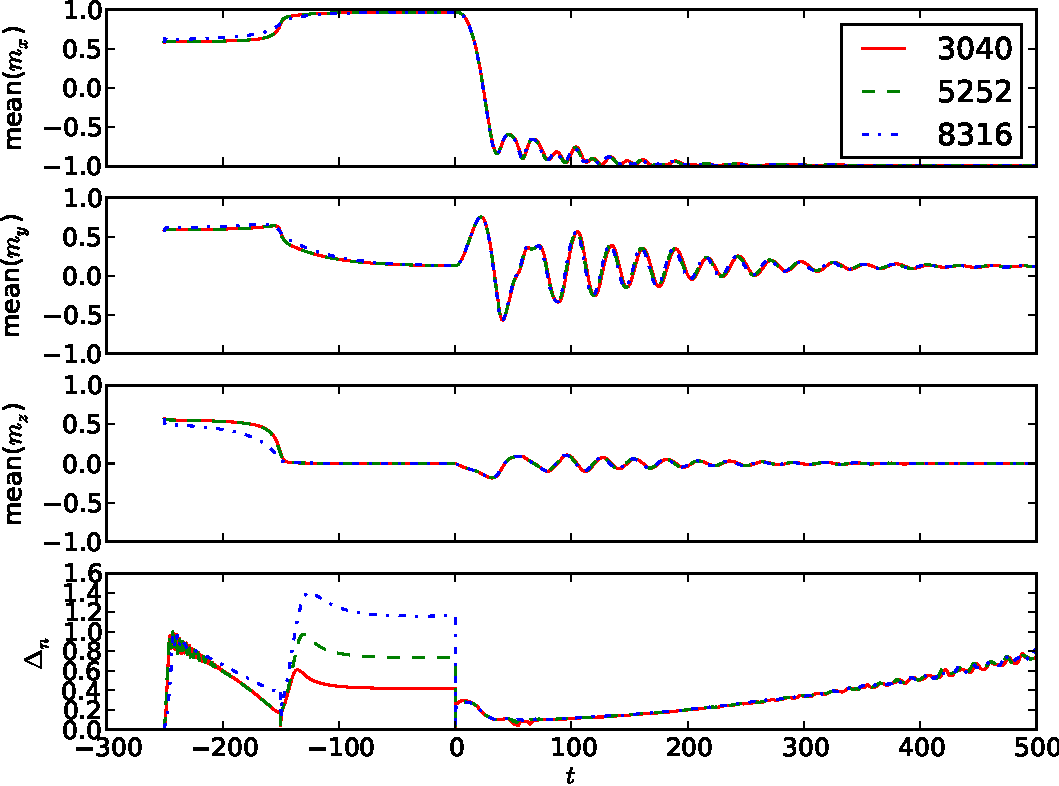
\includegraphics[width=0.8\textwidth]{plots/mumag4_convergence/mumag4_field1-meanmxsvs-meanmysvs-meanmzsvs-dtsvstimes.pdf}
  \caption{Mean magnetisation vs time for field 1 using monolithic IMR with nodal quadrature, the legend shows the number of nodes in the problem.
    ??ds with the results given by nmag and some FD results?}
  \label{fig:nmag-comparison-mumag4-field1}
\end{figure}

\begin{figure}
  \centering
  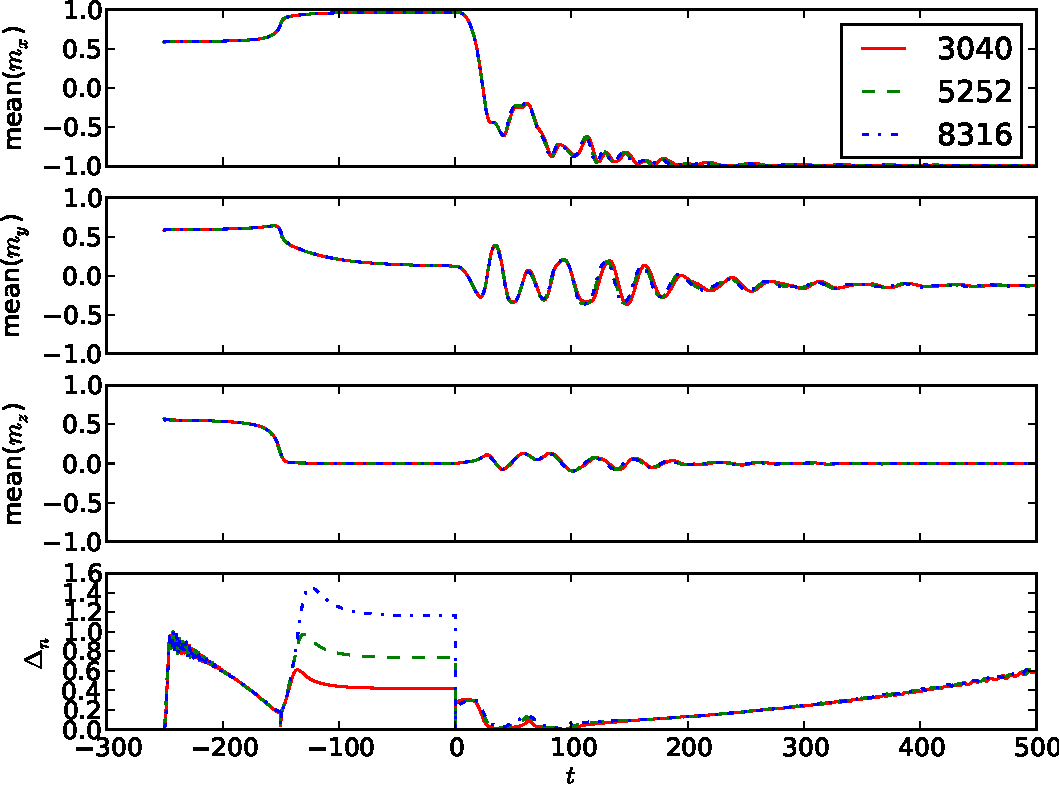
\includegraphics[width=0.8\textwidth]{plots/mumag4_convergence/mumag4_field2-meanmxsvs-meanmysvs-meanmzsvs-dtsvstimes.pdf}
  \caption{Mean magnetisation vs time for field 2 using monolithic IMR with nodal quadrature, the legend shows the number of nodes in the problem.
    ??ds with the results given by nmag and some FD results?
  }
  \label{fig:nmag-comparison-mumag4-field2}
\end{figure}


??ds
Also the state of the system at the time when $m_x$ crosses zero for field 2 is shown in \cref{fig:mumag4-spatial-x-crossing-0}.

\begin{figure}
  \centering
  
\includegraphics[width=0.8\textwidth]{images/placeholder}
  \caption{The state of the system at the time when $m_x$ crosses zero}
  \label{fig:mumag4-spatial-x-crossing-0}
\end{figure}


Since the second field gives a more challenging test, for the rest of the results we only show that field.

We show a comparison of the magnetisation generated using IMR, nodal integration and monolithic or decoupled approach in \cref{fig:mumag4-spatial-x-crossing-0}.
The dynamics are very similar but the monolithic method is able to take larger time steps and suffers from less noise in the size step during the initial relaxation.
\begin{figure}
  \centering
  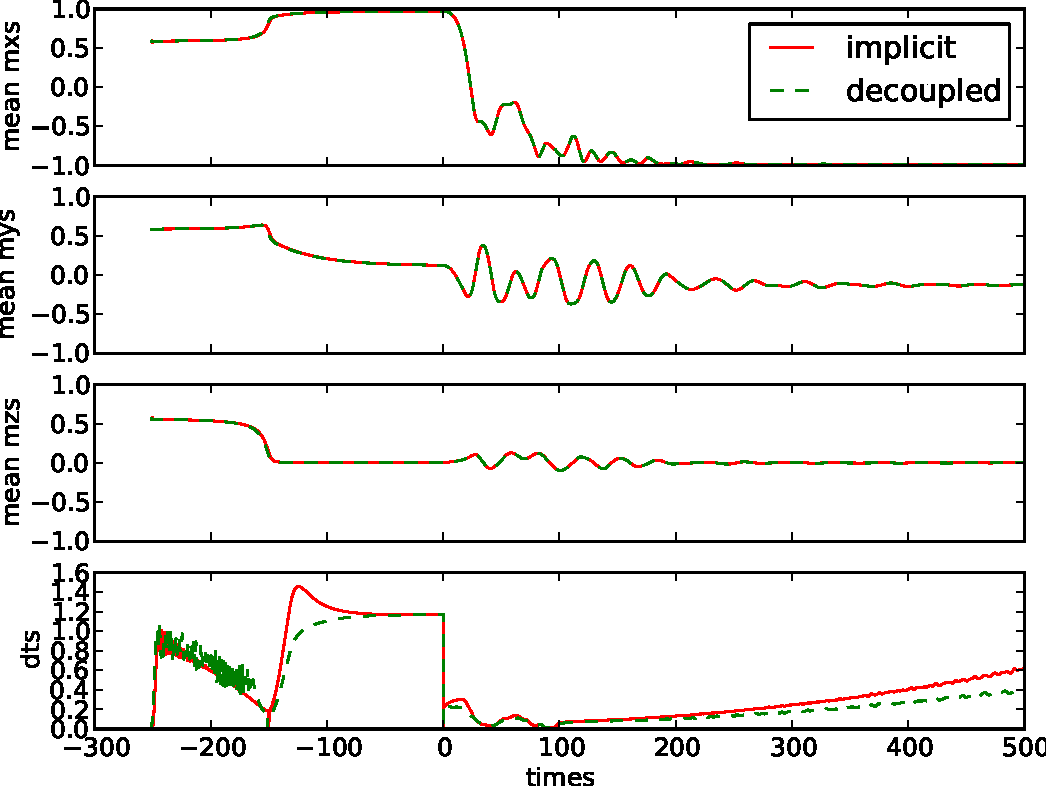
\includegraphics[width=0.8\textwidth]
  {plots/monolithic_vs_decoupled/meanmxsvs-meanmysvs-meanmzsvs-dtsvstimes.pdf}
  \caption{Mean magnetisation vs time for field 2 as computed by the monolithic and decoupled methods with IMR, nodal quadrature and the highest mesh resolution.}
  \label{fig:mumag4-implicit-decoupled}
\end{figure}

\subsection{Geometric integration properties}

The evolution of the maximum nodal error in the magnetisation length for the decoupled and implicit methods is shown in \cref{fig:mumag4-implicit-decoupled}.
As expected both coupling approaches conserve $\abs{\mv}$ to around the Newton tolerance.
\begin{figure}
  \centering
  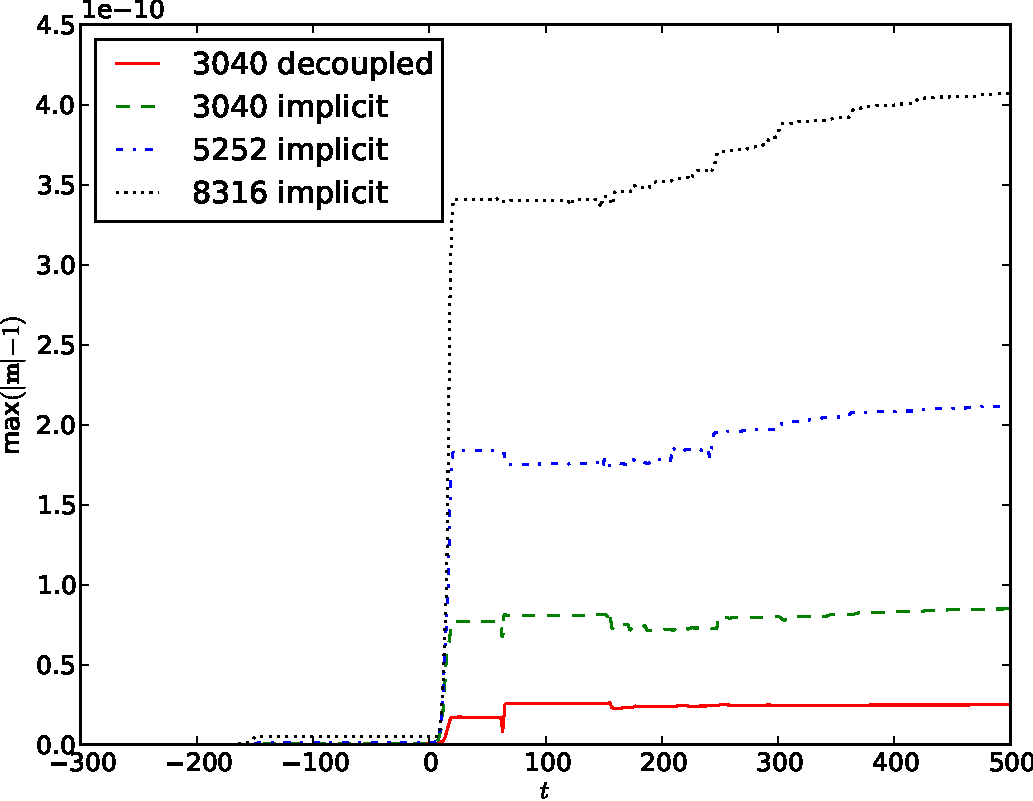
\includegraphics[width=0.8\textwidth]{plots/mumag4_ml/mlengtherrormaxesvstimes.pdf}
  \caption{Magnetisation length errors when using IMR with nodal integration for field 2, legend shows the coupling strategy. ??ds remove extra nnode lines, add Gaussian Q lines}
  \label{fig:imr-conservation}
\end{figure}


The behaviour of the energy when $\dampc = 0$ is shown in \cref{fig:energy-conservation}.
It can be seen that neither the monolithic or decoupled methods give the desired conservation behaviour.
From various other experiments we have drawn the conclusion that this occurs when the magnetostatic calculations are introduced, but we are not sure of the cause.
It should be noted that in the results presented by d'Aquino \cite{DAquino2005} the energy conservation is not as good as would be expected with a Newton tolerance of $10^{-14}$, so it is possible that this is an underlying issue with the IMR.

\begin{figure}
  \centering
  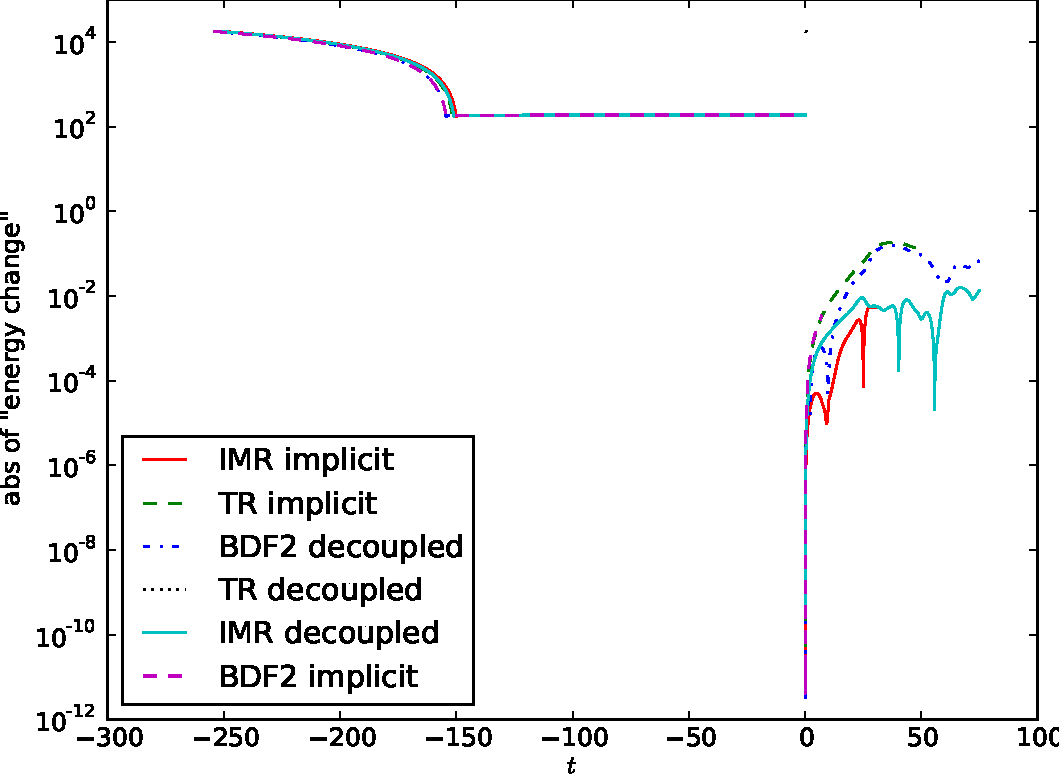
\includegraphics[width=0.8\textwidth]
  {plots/sq_mumag4_energy_conservation/absofenergychangevstimes.pdf}
  \caption{Energy errors for the undamped case.}
  \label{fig:energy-conservation}
\end{figure}


\subsection{Effectiveness of the linear and non-linear solver}

Next we examine the effectiveness of the linear solver for the monolithic method.
The iterations needed for convergence are shown in \cref{fig:mumag4-solver-iterations}, note that while they increase with the number of nodes, $\Nn$, they remain reasonable for the problem sizes required here.
The time taken to set up the preconditioner is displayed in \cref{fig:mumag4-solver-time}, again it grows with the number of nodes but remains reasonable for all cases shown here.
Also note that with nodal quadrature the preconditioner is cheaper to set up but less effective, to counteract this a higher level of fill-in could be used with nodal quadrature.

\begin{figure}
  \centering
  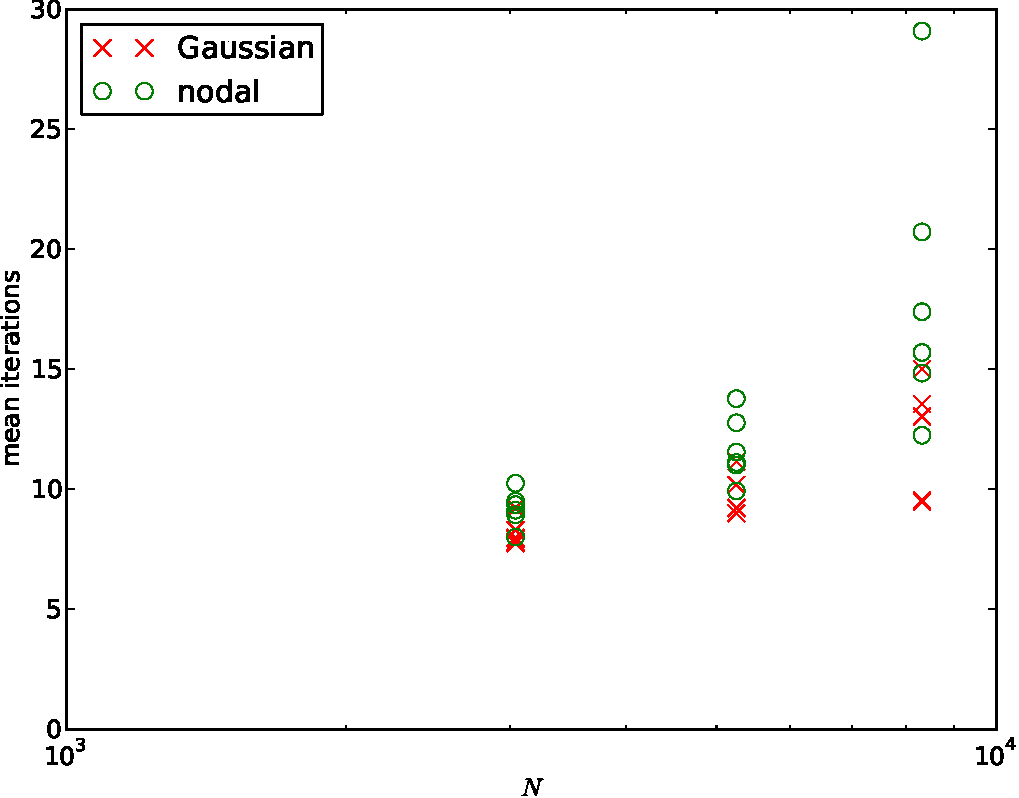
\includegraphics[width=0.8\textwidth]
  {plots/mumag4_monolithic_its/meanofnsolveritersvsinitialnnode.pdf}
  \caption{Mean iterations to converge over all time steps and newton steps for all time steppers and fields using monolithic coupling with GMRES preconditioned by $\inexact{\precc}$.}
  \label{fig:mumag4-solver-iterations}
\end{figure}

\begin{figure}
  \centering
  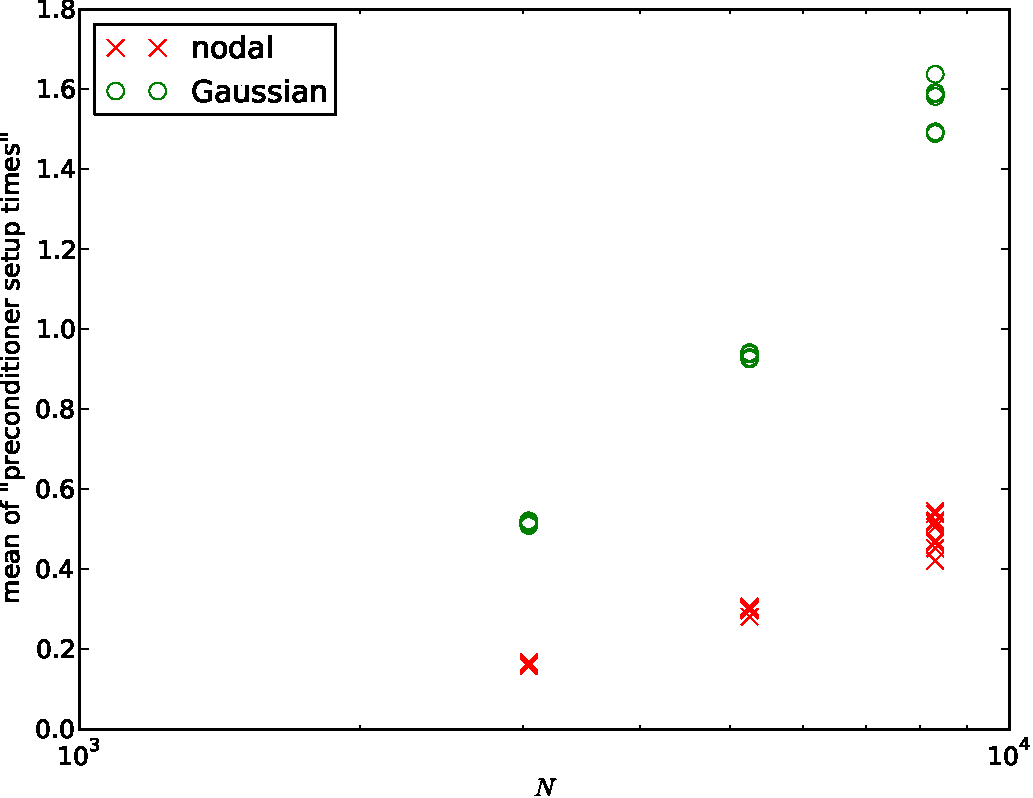
\includegraphics[width=0.8\textwidth]{plots/mumag4_monolithic_its/meanofpreconditionersetuptimesvsinitialnnode.pdf}
  \caption{Mean times to set up the preconditioner $\inexact{\precc}$ against the number of nodes.}
  \label{fig:mumag4-solver-time}
\end{figure}


??ds characterise number of newton steps?


We do not explore the total solve time of the various methods because, due to the lack of hierarchical matrices and the extremely large number of boundary nodes, the solve times are dominated by the BEM matrix and are meaningless for practical problems in which the FEM/BEM method is appropriate.
??ds -- this doesn't seem to be true, need to make some plots :(


\subsection{Conclusions}

Our methods give results for the \mumag problem \#4 which converge well and match up with the results of other FEM/BEM models.
We observe the expected conservation of magnetisation length with IMR and nodal quadrature, but not the expected conservation of energy.



%%% Local Variables:
%%% mode: latex
%%% TeX-master: "main"
%%% End:
